% Paper on velociraptor, a GPU implementation of the likelihoods of TRICERATOPS.
% Each number carries a "% source:" comment: a file of this package (benchmarks/, validation/), a public reference,
% or the author's records, for a measurement whose record is not part of the package.
% The comments never reach the PDF.
\documentclass[11pt]{article}
\usepackage[margin=1in]{geometry}
\usepackage{amsmath}
\usepackage{booktabs}
\usepackage{longtable}
\usepackage{array}
\usepackage{graphicx}
\usepackage{setspace}
\usepackage[hidelinks]{hyperref}
\hypersetup{pdftitle={velociraptor: exact light curves and GPU-accelerated false-positive probabilities for TESS planet candidates}, pdfauthor={Mauri de Souza Meneguzzo}}
\setstretch{1.1}

\title{velociraptor:\\ exact light curves and GPU-accelerated false-positive probabilities for TESS planet candidates}
\author{Mauri de Souza Meneguzzo\thanks{ORCID: \href{https://orcid.org/0009-0000-0032-3262}{0009-0000-0032-3262}}}
\date{}

\begin{document}
\maketitle

\begin{abstract}
% source: author's records; each number is sourced where it is stated in the body.
TRICERATOPS computes the probability that a transit candidate is a false positive by averaging likelihoods over prior draws. We present velociraptor, a GPU implementation of its three likelihood functions that leaves the draws, the priors and the probabilities unchanged. The transit light curve is the closed form of Agol, Luger and Foreman-Mackey on the exact Kepler orbit, in Triton kernels with a single-precision first pass. It agrees with 50-digit references to $2.78\times10^{-16}$ in the lens area and $6.34\times10^{-14}$ in the orbit with NumPy 1.26.4. The light curve of PyTransit 2.2.0, which TRICERATOPS uses, departs from a 50-digit reference by $4.5\times10^{-4}$ to $4.1\times10^{-3}$ on the draws that carry the evidence of some short, eccentric orbits, outside the range in which its authors tested it. On 158 search candidates, the exact model shifts the false-positive probability (FPP) or the nearby-star probability by at least one seed scatter on 15, and moves FPP across a decision value on 2. At $10^{6}$ draws the shifts persist on three of four stars. One calculation of $10^{5}$ draws takes 0.4 to 0.8 s on a consumer card, against 1.5 to 5.5 s for the published code on 32 CPU threads; 20 runs of $10^{6}$ draws take 88 to 105 s, against an extrapolated 661 to 891 s. The package also reports the scatter of the probabilities between seeded batches. Out of sample it covered the truth in 0.667 of trials on six stars, so the package states no coverage for it.
\end{abstract}

\section{Introduction}

A transit candidate is validated statistically when the probability that it is a false positive is small. TRICERATOPS \cite{giacalone2021} computes this probability for a target from the evidence of a set of scenarios: the target hosts a transiting companion, the target or a neighbour hosts an eclipsing binary, a background star does, and so on. The evidence of each scenario is a mean of the likelihood of the light curve over draws from the prior of the scenario's parameters. The probabilities FPP and NFPP follow from the normalised evidences. A candidate is validated when FPP is below 0.015 and NFPP below 0.001 \cite{giacalone2021}. TRICERATOPS validated 12 objects of interest in a vetting of 384 TESS objects of interest \cite{giacalone2021} and 64 further TESS planets in a recent survey of 443 candidates \cite{collier2026}. Other tools compute such probabilities by other means: VESPA \cite{morton2012,morton2016} simulates a population of instances of each false-positive scenario, PASTIS \cite{diaz2014} compares hypotheses by a Bayesian model comparison, and BLENDER \cite{torres2011} models the photometry as blend scenarios.
% source: Giacalone et al. 2021 (reference 1) for the criteria and the 12 validated of 384; Collier et al. 2026 (arXiv:2608.21560) abstract: 443 candidates, 64 new validated planets; Morton 2012 (ApJ 761, 6; arXiv:1206.1568), Morton et al. 2016 (arXiv:1605.02825), Diaz et al. 2014 (arXiv:1403.6725), Torres et al. 2011 (arXiv:1008.4393), from their arXiv pages.

The light curve of the transit must be right on the orbits of the draws, including short and eccentric ones. The speed must fit the published practice: Collier et al.\ \cite{collier2026} run the calculation 20 times per target, each run with its own seed and $10^{6}$ draws, and Giacalone et al.\ \cite{giacalone2021} chose $N=10^{6}$ as the number of draws that gives results consistent between consecutive calculations (their Section 2.4) and repeated the calculation 20 times for each of their 12 validated objects (their Section 6). The Monte Carlo also needs a statement of how far it can be trusted, since the scatter of FPP between seeds depends on the star (Section~\ref{sec:stating}).
% source: arXiv:2608.21560v3 (Collier et al. 2026), Section IV.6.1 ("20 independent runs per target, each with a distinct random seed and each drawing 10^6 Monte Carlo samples") and the abstract (443 candidates, 64 newly validated planets), read from the arXiv HTML; arXiv:2002.00691v2 (Giacalone et al. 2021), Section 2.4 (N = 10^6) and Section 6, the paragraph that introduces Table 6 (20 runs for each of the 12 validated TOIs); both read from the texts.

velociraptor replaces the three likelihood functions of TRICERATOPS 1.1.0 with a calculation on a graphics processor and leaves the draws, the priors and the probabilities unchanged. Its transit light curve is the closed form of Agol, Luger and Foreman-Mackey \cite{agol2020} on the exact Kepler orbit. Section~\ref{sec:design} describes the design, Section~\ref{sec:accuracy} the accuracy against references, Section~\ref{sec:agreement} the agreement with the published code and the stars on which they differ, Section~\ref{sec:performance} the time and memory, and Section~\ref{sec:stating} the scatter between seeded batches that the package reports and what was measured about it. Section~\ref{sec:limits} lists what was not verified.

\section{Design}\label{sec:design}

\subsection{The calculation}

For each scenario TRICERATOPS draws $N$ parameter vectors from the prior, computes a model light curve for each, forms the chi-squared against the folded light curve, and takes the evidence as the mean of $\exp(-\chi^2/2)$ times the prior-volume factors of the scenario. The light curve is a quadratic limb-darkened transit \cite{mandel2002} on a Keplerian orbit, integrated over the exposure. Throughout, the published code is TRICERATOPS 1.1.0 with its default settings and its transit model, PyTransit 2.2.0 \cite{parviainen2015}.

\subsection{The exact model}

The flux removed by the planet is the integral of the stellar intensity over the part of the planet's disc inside the star. velociraptor evaluates it by the closed form of Agol, Luger and Foreman-Mackey \cite{agol2020}, which writes the integral with complete elliptic integrals, and by a second implementation after Mandel and Agol \cite{mandel2002}, a Gauss--Legendre quadrature of the arc of the planet's disc inside each ring of the star, used as a cross-check. Where the planet is small and wholly inside the stellar disc, which is nearly every element of a calculation, the flux is a series in the radius ratio, the mean of the intensity over the planet's disc (Pizzetti's series for the mean value of an analytic function), of order 3 or 9 chosen from a bound on the first omitted term, so that no elliptic integral is evaluated there. The orbit is the exact Kepler orbit: Kepler's equation is solved for each point of each exposure, with no Taylor expansion about mid-transit.
% source: velociraptor package docstrings of its closed-form, series and quadratic modules (the closed form of Agol, Luger and Foreman-Mackey; the quadrature of Mandel and Agol after the substitution r = m - h cos(phi); Pizzetti's series; orders 3 and 9 chosen by a bound on the first omitted term at a tolerance of 1e-14 in absolute flux), author's records.

\subsection{The device kernels}

The kernel is written in Triton and runs on ROCm and CUDA devices. Each lane handles one pair of a draw and a point: Kepler's equation and the sky separation for each exposure sub-sample, then the flux. The complete elliptic integrals are evaluated by Bulirsch's algorithm in at most 8 steps of the Landen recurrence, left as soon as every lane of the block has converged. A block of 32 lanes with no sub-sample over the stellar disc skips the closed form.

The kernel has two passes. The first pass forms, for each exposure node, the small change of the eccentric anomaly from the centre of the exposure (a few Newton steps on an angle of at most 0.1 rad) and the order-3 series flux of a small planet wholly inside the disc, as a deficit, in single precision. It flags a pair for the second pass when a node is not on the series (ingress and egress, a larger planet, the band within $10^{-4}$ of the contact $b+k=1$) or when the exposure moves the anomaly by more than 0.1 rad. The orbit of the centre, the weights, the tests, the sum into the flux and the second pass, the closed form for the flagged pairs, are in double precision. A guard at the outer contact keeps a lane that lies just inside the contact in double precision from rounding outside it in single precision (Section~\ref{sec:fp32}).

The kernel is launched in slices of at most $2^{20}$ sub-sample elements, so that no dispatch runs long enough to starve the display or trip the driver's ring timeout; the slice is a multiple of 32 pairs, so the blocks, and with them the last bits of the flux, do not depend on the slice size.
% source: velociraptor package docstrings of the kernel, the mixed-precision first pass and the launch plan (two passes; float32 and float64 parts; flag conditions; guard; slices of at most 2^20 elements, multiples of 32; CEL_STEPS = 8).

The exposure is integrated with 3 Gauss--Legendre nodes by default and with the 20 equal parts of the published code as an option. The default is a different quadrature from the published code's, with its own difference from the 20 midpoints (Section~\ref{sec:fp32}). Throughout this paper the default is the call \texttt{install("cuda")} with no further arguments: the Triton kernel, 3 exposure nodes and the single-precision first pass, with the overlap of 3 scenario calls.

\subsection{Integration with TRICERATOPS}

\texttt{install} puts the package's functions in place of TRICERATOPS's three likelihood functions for the length of a block and puts them back on leaving it. Three further pieces handle the host.

First, the splines of TRICERATOPS that sample a scenario hold the interpreter lock through scipy's evaluation, which prevents the sampling of one scenario from overlapping that of the next. velociraptor evaluates them with the recurrence of de Boor, with the same operations in the same order, compiled without the lock; the values are the same to the last bit. Second, the overlap: \texttt{calc\_probs} calls its scenario functions in a fixed order and each draws all its random numbers before its first likelihood call, so the sampling of the next scenario can begin once the likelihood of the one before has begun. Inside the overlap block \texttt{calc\_probs} runs once with stand-ins that record the calls, and then for real with the recorded calls run by worker threads in order; the draws, their order and the results are those of the sequential run bit for bit, and the overlap is given up and the sequential run done if the recorded and real calls differ. Third, TRICERATOPS draws every scenario from one global random stream, so leaving one scenario out changes the numbers of all the others; \texttt{scenario\_streams} gives each call a stream fixed by the seed, the function and the index of the call.

The seeded batches of Section~\ref{sec:stating} seed numpy's one global generator for each batch, which concurrent calls would share. The package therefore runs the calls of a batch one at a time and suspends the overlap inside \texttt{batches}, so batches cost the time that the overlap saves.
% source: velociraptor package docstrings of the install, spline, overlap and stream modules.

\subsection{Stars}\label{sec:samples}

Table~\ref{tab:samples} lists the stars used and the rule that chose each set. The criteria of each comparison of Sections~\ref{sec:agreement} and~\ref{sec:stating}, what counts as a shift, a change of side, a persistence or a coverage, and the hypotheses tested, were fixed before its measurements were made. 
The stars of the screen set are TESS targets on which a periodic transit search of the light curve found a signal above its detection threshold and which were then passed to TRICERATOPS. They are candidates of a search and not a random sample of stars.
% source: author's records (the stored calculations of the stars, made for the signals that a transit search found above its threshold) and the data trace of Section~\ref{sec:limits} (the light curve and product recorded for 136 of the 159 stars, the other 23 from two earlier runs of the same search); the sentence states how the stars came to a calculation and nothing about their number of signals or their nature.
% source: author's records (the sizes and the selection rules of each set).

\begin{table}[ht]
\centering
\caption{The stars used. A hash order is the ascending order of the SHA-256 of a fixed string and the TIC identifier of the star.}\label{tab:samples}
\footnotesize
\begin{tabular}{>{\raggedright\arraybackslash}p{2.4cm}r>{\raggedright\arraybackslash}p{7.2cm}>{\raggedright\arraybackslash}p{3.2cm}}
\toprule
Set & stars & Selection rule & Used in \\
\midrule
% source: author's records (four stars of the precision and speed rows).
Precision and speed stars & 4 & TIC 396212145, 206361339, 42071226 and 201354238, the stars of the benchmark of the package, with no selection rule beyond the availability of their stored tables; the first two carry the tolerance test. & Sections~\ref{sec:accuracy}, \ref{sec:performance} \\
% source: author's records (159 stars in three strata; 158 run: 45 flagged and all 113 unflagged).
Screen set & 159 & The stars with a stored TRICERATOPS table in earlier calculations: 45 flagged by a screen (the best draw of a scenario of probability at least 0.1 has eccentricity above 0.5 and scaled semi-major axis below 15), 113 not flagged, 1 unscreened. Each stratum is taken in a hash order. The comparison of the two models of Section~\ref{sec:model} ran on 158 of them, the 45 flagged and all 113 not flagged; one further star was excluded because TRICERATOPS refused it, and one is unscreened and was not run. & Section~\ref{sec:model} \\
% source: author's records (six stars by hash order with FPP scatter over 1e-3, four stars of the in-sample coverage measurement excluded; 100 batches of 1e5 draws).
Coverage stars & 6 & The first six stars in hash order whose FPP scatter over ten seeds exceeds $10^{-3}$, excluding the four stars of the in-sample coverage measurement; 100 batches of $10^{5}$ draws. & Section~\ref{sec:stating} \\
\bottomrule
\end{tabular}
\end{table}

\section{Accuracy}\label{sec:accuracy}

\subsection{Against references}

Against references that do not come from the package the closed form differs by at most $2.78\times10^{-16}$ from the lens area in 50 digits without limb darkening (552 cases), $1.52\times10^{-13}$ from a two-dimensional integral (10 cases) and $6.44\times10^{-15}$ from 768 nodes of the quadrature (3,312 cases), and the sky separation of an orbit differs by at most $6.34\times10^{-14}$ with NumPy 1.26.4 from a 50-digit solution (9 cases).
% source: validation/results.json, keys lens_area (552 points, largest 2.78e-16 at k = 3), two_dimensional_integral (10 radius ratios, largest 1.52e-13), convergence (3,312 points, largest 6.44e-15 against 768 nodes) and orbit_50_digit (9 eccentricities, largest 6.34e-14 under numpy 1.26.4, the documented install; 3.92e-13 under numpy 2.5.4).

\subsection{The exposure integral}

In these four calculations the 3-node default agrees with the integral of 64 nodes at the same seed: its FPP differs by at most $9.1\times10^{-6}$ and its NFPP by at most $1.0\times10^{-5}$, which is at most 0.003 of the scatter of FPP or NFPP between ten seeds of the 3-node default on each star.
% source: author's records (3-node FPP error 2.53e-06, 9.06e-06, 1.01e-06 and NFPP error 2.49e-06, 1.01e-05 against 64 nodes at the same seed; 0.000 to 0.003 of the seed scatter).

\subsection{Single precision}\label{sec:fp32}

\paragraph{The first pass.} The mixed-precision kernel forms the times relative to mid-transit, the flux as a deficit, sums the chi-squared in double precision and evaluates the closed form near contact in double precision. A second variant evaluates the closed form in single precision as well, with a guard at the outer contact. The flux of the closed form in single precision differs from double precision by at most $3.6\times10^{-7}$ over radius ratios 0.003 to 1.7 and four limb-darkening laws, and by at most $3.3\times10^{-7}$ on the nodes of a planet row, against the rule of $10^{-6}$. Without the guard, a lane just inside the outer contact in double precision can round outside it in single precision, and the flux is wrong by up to 9. The cause is rounding across a branch and not a loss of precision in the formula.
% source: author's records (single-precision closed form 3.6e-7 over radius ratios 0.003 to 1.7 and four laws; 3.3e-7 on the nodes of a planet row; failure up to 9 without the guard).

\paragraph{Shift of the probabilities.} Table~\ref{tab:shift} gives the largest shift in any $\ln Z$ and the shift in FPP of the single-precision first pass against double precision, at 20 midpoints, on four stars. The shifts of FPP are $5.6\times10^{-7}$ to $4.6\times10^{-6}$ where FPP is not pinned. On the two stars with a stored seed scatter the smallest scatter of the $\ln$ probability of a scenario is 7.2 and 0.7, against largest shifts of 0.0185 and $2.5\times10^{-4}$. No probability changes side of 0.015 or 0.5.
% source: author's records (largest shifts of ln Z and of FPP of the single-precision first pass) and the author's records (seed scatter of the ln probability: smallest 7.2 and 0.7).

\begin{table}[ht]
\centering
\caption{Shift of the evidence and of the probabilities from a single-precision first pass against double precision, whole calculation at the 20-midpoint exposure integral.}\label{tab:shift}
\begin{tabular}{lrrr}
\toprule
TIC & largest shift of $\ln Z$ & shift of FPP & shift of $\ln\mathrm{NFPP}$ \\
\midrule
% source: author's records, shifts of the single-precision first pass against double precision.
396212145 & 0.0185 & 0 (FPP 1) & $5.4\times10^{-5}$ \\
206361339 & $2.5\times10^{-4}$ & $4.6\times10^{-6}$ & $6.4\times10^{-5}$ \\
42071226  & $8.8\times10^{-6}$ & $5.6\times10^{-7}$ & $1.5\times10^{-6}$ \\
201354238 & $2.5\times10^{-5}$ & $1.9\times10^{-6}$ & (NFPP 0) \\
\bottomrule
\end{tabular}
\end{table}


The default of the package is the 3 nodes with the single-precision first pass, and it was checked as a default on the four stars of Table~\ref{tab:time}, each at eight seeds of 100,000 draws, against the same calculation in double precision at 3 nodes. The largest shift of any $\ln Z$ is 0.32 percent of the seed scatter of its row, against a limit of 10 percent; the sides of FPP $=0.015$ and $0.5$ and of NFPP $=10^{-3}$ agree at every seed; the largest differences are $1.3\times10^{-4}$ in FPP and $1.1\times10^{-4}$ in NFPP, both on one star. On one star three of 18 rows are $-\infty$ in both precisions at every seed and carry no test. The default is 1.09 to 1.59 times faster than double precision at 3 nodes (Table~\ref{tab:time}).
% source: author's records (the 3-node check of the mixed default: worst shift 0.0032 of the row's scatter against 0.1; sides agree at 8 seeds; FPP 1.3e-4 and NFPP 1.1e-4; 3 of 18 rows -inf in both on TIC 396212145) and the author's records (the times of Table 5: 0.614 to 0.483, 0.419 to 0.383, 0.715 to 0.545, 1.230 to 0.776).


\paragraph{A kernel in single precision only.} The single-precision closed form is measured as a function of the radius ratio, the limb darkening and the distance from contact, with the largest error given above. Whether a kernel with no double precision at all meets the rule of $10^{-6}$ in flux is not settled. On the benchmark's draws the error is within it up to periods of about 3 days and reaches $3.5\times10^{-6}$ at 30 days, growing with the semi-major axis in stellar radii, which points at the rounding of the orbit. Such a kernel is not built.
% source: author's records (a kernel with no double precision: within 1e-6 up to about 3 days, 3.5e-6 at 30 days).


\subsection{The precision the probabilities need}\label{sec:precision}

The probabilities are insensitive to errors in the flux of the size that single precision makes. On two stars, one with FPP pinned at 1 and one with FPP 0.090, we added an error to the light curve and found the largest error at which every scenario whose scatter between ten seeds exceeds $10^{-3}$ shifts by less than a tenth of its scatter, and $\ln\mathrm{NFPP}$ likewise. An absolute flux error that is independent for each element is tolerated at $10^{-7}$ and not at $10^{-6}$. A relative error in the deficit $1-F$ is tolerated at $10^{-3}$ and not at $10^{-2}$. At the largest tolerated level the largest shift is 0.11 of the limit for the flux (at $10^{-7}$) and 0.25 for the deficit (at $10^{-3}$); at the next level it is 1.07 and 2.46. The FPP of the star at 0.090 moves by $6.3\times10^{-3}$ under a flux error of $10^{-6}$ and by $9.5\times10^{-4}$ under a deficit error of $10^{-3}$, against its scatter of 0.17. Rounding the flux to single precision shifts the probabilities by 0.004 of the limit, and rounding the deficit by $3.5\times10^{-6}$ of it. The rounding is a deterministic function of the flux and not an independent error, and its shift is smaller than that of an independent error of the same size.
% source: author's records (tolerances 1e-7 / 1e-6 and 1e-3 / 1e-2; ratios 0.11, 1.07, 0.25, 2.46; single-precision rounding 0.004 and 3.5e-6 of the limit; FPP 0.090 shifts 6.3e-3 and 9.5e-4 against scatter 0.17).

The tolerance holds for independent errors. A systematic error, such as the bias of an orbit approximation that is the same on every draw, adds over the points of the light curve and has a lower tolerance. It is also relative to the scatter at $10^{5}$ draws, and a run with more draws has a smaller scatter and a tighter tolerance.
% source: author's records, limits of the measure.


\section{Agreement with the published code, and where they differ}\label{sec:agreement}

The two calculations draw the same parameters and form the same chi-squared, so the probabilities differ only where the two light curves differ on the draws that carry the evidence of a call. On the heaviest draw of the control call of a star that did not shift the two curves agree, and so do the probabilities. Where the heaviest draw of a call is a draw on which the curves differ, FPP may move; agreement on the published code's heaviest draw is not enough, because the exact calculation may weight another draw most, as on TIC~42071226 (Section~\ref{sec:model}).
% source: author's records (the control call: the heaviest draw not an affected draw; TIC 42071226 3e-9).

\subsection{Where the published transit model differs}\label{sec:model}

The light curve of PyTransit 2.2.0, which TRICERATOPS 1.1.0 uses, departs from the exact light curve on some orbits. Section~\ref{sec:design} gives the exact orbit and the closed form of the package. We swept a grid of 320 parameter sets, not drawn from a population: four periods (0.5, 0.713, 2 and 10 d), five scaled semi-major axes (3, 4, 6, 10 and 20), four eccentricities (0, 0.3, 0.5 and 0.7) and four arguments of periastron. In 70 of the 320, PyTransit's model puts a second dip, a flux under $1-10^{-6}$ where the exact flux is 1, at 0.004 to 0.25 of the period from mid-transit: in none of the 80 sets at zero eccentricity, 10 of the 80 at 0.3, 24 at 0.5 and 36 at 0.7. The flux of the model is off the exact one by more than $10^{-5}$ in 143 of the 320.
% source: author's records (the grid of 320 parameter sets, 4 x 5 x 4 x 4; the 70 with a second dip: 0, 10, 24 and 36 of 80; 143 off by more than 1e-5; the second dip at 0.004 to 0.25 of the period).

The validation of the package compares the two models on 300 further orbits, drawn at random with periods of 0.5 to 30 d, $a/R_\star$ of 2 to 40 and eccentricities of 0 to 0.9. For $a/R_\star$ of 20 to 40 and eccentricities under 0.3 the median of the largest flux difference of an orbit is $5.0\times10^{-9}$. At eccentricities over 0.6 the largest difference is 0.078 for $a/R_\star$ of 5 to 10 and 0.17 for the one orbit with $a/R_\star$ under 3.
% source: validation/results.json, key pytransit_orbits (300 orbits drawn with seed 1; cells a/R* 20-40, e <0.3: median 4.99e-9 over 54 orbits; a/R* 5-10, e >0.6: largest 0.0779 over 11; a/R* <3, e >0.6: 0.169, one orbit); the draws of validation/pytransit_grid.py.

One orbit of that comparison gives a minimal reproduction. Take $P=21.99247$~d, $a/R_\star=6.964572$, an inclination of $87.04449^{\circ}$, $e=0.8502341$, $\omega=347.7677^{\circ}$, $k=0.4962705$, quadratic limb darkening $(u_1,u_2)=(0.4,0.25)$ and mid-transit at $t=0$. At $t=-0.7894$~d, with a 30-minute exposure evaluated at its centre, the \texttt{QuadraticModel} of PyTransit 2.2.0 with \texttt{interpolate=False} gives a flux of 0.92212, where the planet is off the stellar disc and the exact flux is 1.
% source: validation/pytransit_grid.py, orbits(), the draw of index 76 of 300 with seed 1 (the largest difference, 0.07788, of the cell a/R* 5-10, e > 0.6 of validation/results.json key pytransit_orbits), rerun in the PyTransit environment of validation/pytransit_env.md: PyTransit 0.9221220357 and velociraptor transit_flux 1 at t = -0.7894408565 d.

\paragraph{The size of the shift in FPP.} On four stars, the FPP of the published code differs from that of the exact calculation on the same draws by 5.8 and 7.7 seed scatters on two of them (1.0000 against 0.9024, and 0.7376 against 0.7725) and agrees on the other two. Four stars give no rate, so we compared the two models on the 158 stars of the screen set of Table~\ref{tab:samples} that were run: 45 flagged by the screen and 113 not flagged, in hash order within each stratum. Each calculation, with 100,000 draws, ran under both models on the same draws at three seeds, and under the exact model at ten seeds, whose standard deviation of FPP is the seed scatter. The exact model ran in double precision with the 20 exposure midpoints of the published code, so the two calculations differ in the light curve alone and not in the quadrature or the precision. Appendix~\ref{sec:stars} lists the stars with their FPP under both models. A star is shifted in FPP if the mean difference of FPP between the two models is at least the larger of that scatter and 0.01 and has that size and sign at each of the three seeds; in $\ln\mathrm{NFPP}$ the same with a floor of 0.095, counted only where NFPP is at least $10^{-3}$ in one of the models.
% source: author's records (the screen and the 158 stars; 100,000 draws; the exact arm in float64 at 20 midpoints, exposure_nodes=None, three calls in flight; three seeds for the published code and ten for velociraptor; the rule of a shifted star).

Of the 45 flagged stars 5 are shifted in FPP (11 percent, Wilson 95\% interval 4.8 to 23.5 percent) and none in $\ln\mathrm{NFPP}$. Of the 113 unflagged stars, which are all the unflagged stars of the set, 10 are shifted (8.8 percent, 4.9 to 15.5 percent), 6 in FPP and 5 in $\ln\mathrm{NFPP}$, one in both. Over the 158 stars 15 are shifted (9.5 percent, 5.8 to 15.1 percent). The interval of the unflagged share includes the point value of the flagged share, so the screen does not separate the stars that shift. Over the 11 stars shifted in FPP, the published code's FPP is higher on 8 and lower on 3 (a two-sided sign test gives $p$ of about 0.23); the direction is observed here, and no direction is claimed in general. The hypothesis that stars of low noise per point shift more is not supported: 3 of 50 stars shifted in the lowest third of the noise and 8 of 50 in the highest (one-sided Fisher $p=0.97$, on the first 150 stars run).
% source: author's records (5 of 45, Wilson 4.8 to 23.5; 10 of 113, Wilson 4.9 to 15.5, 6 in FPP, 5 in ln NFPP, one in both; 15 of 158, Wilson 5.8 to 15.1; the rule of the screen; the published code higher on 8 and lower on 3 of the 11 shifted in FPP; the noise test 3 of 50, 3 of 50, 8 of 50, p = 0.97).

Two stars of the 158 change side of a decision value between the two models (1.3 percent, Wilson 0.35 to 4.5 percent), with the FPP of the published code the lower in both, and none changes side of the NFPP line of $10^{-3}$. Fewer than three stars that change side are stated as cases and not as a rate of changes of class; these are two cases.

The first, TIC~325177252, changes side of FPP $=0.015$. It is not flagged and has a noise per point of $5.0\times10^{-5}$. The FPP of the published code is 0.00028, 0.00020 and 0.0021 at three seeds, all under 0.015, and that of the exact model is 0.026 to 0.038 at ten seeds (scatter 0.0037), all over it; NFPP is under $10^{-3}$ in both. On the criteria of TRICERATOPS itself, the published code would pass the star and the exact model would not.

The second, TIC~424717049, changes side of 0.5 and is the largest shift, 83 seed scatters. It is not flagged and has a noise per point of $2.4\times10^{-3}$. The FPP of the published code is 0.313, 0.0002 and 0.0001 at three seeds and that of the exact model 0.858 to 0.888 at ten. At seed 1 the published code puts 0.62 of the probability on the scenario PTP, 0.31 on STP and 0.06 on the target's planet (TP), while the exact model puts 0.54 on SEB and 0.08 on TP; the scenario names are those of TRICERATOPS.

One further star, TIC~278659026, differs by 23 seed scatters (the published code 1.0, exact model 0.577, both above 0.5).
% source: author's records (2 of 158 changing side, Wilson 0.35 to 4.5 percent, both the published code under, none at the NFPP line; TIC 325177252: noise 5.0e-5, the published code 0.00028, 0.00020, 0.0021, exact 0.026 to 0.038 at ten seeds with scatter 0.0037, NFPP under 1e-3; TIC 424717049: noise 2.4e-3, the published code 0.313, 0.0002, 0.0001, exact 0.858 to 0.888, seed 1 probabilities PTP 0.62, STP 0.31, TP 0.06 against SEB 0.54, TP 0.08; the rule of fewer than three; TIC 278659026 at 23 scatters, 1.0 and 0.577).

\paragraph{Against a reference in 50 digits.} On each of the eight shifted stars replayed we took the call with the largest difference of $\ln Z$ between the models and computed the light curve of the draw that each model weights most against a reference built from Kepler's equation in 50 digits. On the four flagged stars of the first part, the exact curve of velociraptor differs from the reference by at most $2.2\times10^{-16}$ on all eight draws. The curve of the published code differs by $4.5\times10^{-4}$ to $3.0\times10^{-3}$, against a noise per point of $3.5\times10^{-4}$ to $1.8\times10^{-3}$, and half its chi-squared against the data is lower than the reference's by 11 to 32 on the draw that the published code weights most. On two of the four stars the curve of the published code is also off by $8.0\times10^{-4}$ and $4.5\times10^{-4}$ on the draw that the exact calculation weights most, and the data do not prefer it there. On TIC~325177252 the exact curve is within $3.3\times10^{-16}$ of the reference, and the published code is off by $4.1\times10^{-3}$, 80 times the noise, on the draw that both models weight most. On TIC~278659026 the heaviest draws lie in the screened region ($k=0.76$, $e=0.70$, $a/R_\star=6.7$). There the published code is off by about 0.0029 in the flux of the target, against a fold error of 0.0019. The host star of the scenario is a faint neighbour, whose flux and error the package rescales by about 144, and in its flux the error is 0.42 against a fold error of 0.278. The exact curve is within $2\times10^{-15}$ of the reference, and the heaviest draw of the published code lies at the 99.99th percentile of $\Delta$. On TIC~42071226 the heaviest draw of the published code agrees with the reference to $3\times10^{-9}$. On TIC~424717049, call 6 (the STP row, $\ln Z$ differing by $+47.4$), the heaviest draw of the published code ($k=0.095$, $e=0.39$, $a/R_\star=2.26$, inclination $86.0^{\circ}$) is off the reference by $2.15\times10^{-3}$, 0.9 of the noise per point, and the exact curve is within $2.2\times10^{-16}$; half the chi-squared against the data is 424.7 for the published code and 480.8 for the reference. The secondary eclipse of the eclipsing-binary likelihoods is not part of the reference.
% source: author's records (the replay against the 50-digit reference: 2.2e-16; 4.5e-4 to 3.0e-3; noise 3.5e-4 to 1.8e-3; half chi-squared lower by 11 to 32; 8.0e-4 and 4.5e-4; TIC 325177252 3.3e-16 and 4.1e-3, noise 5.0e-5; TIC 278659026 k 0.76, e 0.70, a/R* 6.7, 0.42 and 0.40 against 0.278; TIC 42071226 3e-9).

\paragraph{What makes the shift.} The evidence of a call rests on its heaviest draws. For every draw of the replayed calls on which the two curves differ by more than $10^{-6}$ we computed the difference $\Delta$ of half the chi-squared of the exact curve and of the published code's curve (positive when the published code fits better). The exact curve stands in for the 50-digit reference, from which it differs by at most $4.4\times10^{-15}$ on the heaviest draw and ten affected draws of each call. Each pattern is read from the heaviest draw of the call with the largest difference of $\ln Z$; the direction of the shift in FPP follows from the pattern and from the scenario to which the call belongs.

The first pattern is a favourable error on the heaviest draw. The heaviest draw of the published code is one on which its error happens to fit the data better than the exact curve, so the evidence of the call rises. FPP then rises if the call is a false-positive scenario and falls if it is a planet scenario, as for TIC~424717049. This is the case of a planet call of TIC~403224147, of TIC~278659026 and of TIC~424717049. On the planet call of TIC~403224147 $\Delta$ is centred on zero (median $-0.003$) and the published code fits better on 47.5 percent of the 6,508 affected draws; the heaviest draw of the published code lies at the 99.92th percentile, where the published code fits better by 32.5, which is what a random error of the size of the noise and a maximum over draws would give. On the draw of Figure~\ref{fig:curves} (left), the spurious dip of the published code, about 0.07 d before the transit, falls on a dip of the data, structure that a likelihood with white noise does not model, and the favourable error is a fit to it. This is read from one draw of the planet call. On TIC~424717049 the distribution of $\Delta$ is centred on zero and the heaviest draw of the published code lies at the 99.99th percentile.

The second pattern is a large error of the published code on most draws of an eclipsing-binary call. In TIC~122609480, 405410684 and 340786513, the published code fits better on only 13 to 15 percent of the 4,084 to 12,573 affected draws of the call, with a tail of $\Delta$ to $-1.6\times10^{6}$. The heaviest draw of the published code lies at the 91st to 98.5th percentile ($\Delta$ 11.2, 20.1 and 12.8). The error of the published code is large on most affected draws, and the draw that carries its evidence is one of the few on which it fits, so its evidence is the higher. In TIC~325177252, call 10, an eclipsing-binary call whose $\ln Z$ differs by $-40{,}351$, the heaviest draw is the same in both models ($k=0.80$, $e=0.26$, $a/R_\star=2.46$, inclination $24.6^{\circ}$, period 0.927 d) and the error of the published code removes it, so the published code is lower; half the chi-squared against the data is 236,644 for the published code and 196,294 for the reference (Figure~\ref{fig:curves}, right).

The third pattern is a spoiled exact draw. The error of the published code spoils the draw that carries the evidence of the exact model. This is TIC~42071226, where the heaviest draw of the published code agrees with the reference to $3\times10^{-9}$ and on the heaviest draw of the exact model the published code fits worse by 131 in half chi-squared, so the published code is lower.

In the control call of a star that did not shift, the tail of $\Delta$ is as heavy ($-1.9\times10^{5}$) and the heaviest draw is not an affected draw, so the published code and the exact model agree on it. A shift therefore needs the draw that carries a call to be an affected draw, and its sign depends on whether the error helps the fit of that call and on the scenario of the call. The first two patterns are read on the replayed stars only. How often each occurs for calls whose evidence rests on more draws, and the cause of the error inside PyTransit, are not shown here.
% source: author's records (the Delta of the replayed calls and three controls; TIC 424717049 centred on zero, 99.99th percentile; the exact curve within 4.4e-15 of the reference; planet call median -0.003, 47.5 percent, 6,508 draws, 99.92th percentile, 32.5; EB calls 13 to 15 percent, 4,084 to 12,573 draws, 91st to 98.5th percentile, 11.2, 20.1, 12.8; control tail -1.9e5) and the author's records (the patterns: TIC 42071226 3e-9 and 131; TIC 325177252 call 10, ln Z -40,351, k 0.80, e 0.26, a/R* 2.46, inclination 24.6 degrees, period 0.927 d, half chi-squared 236,644 and 196,294).

\begin{figure}[ht]
\centering
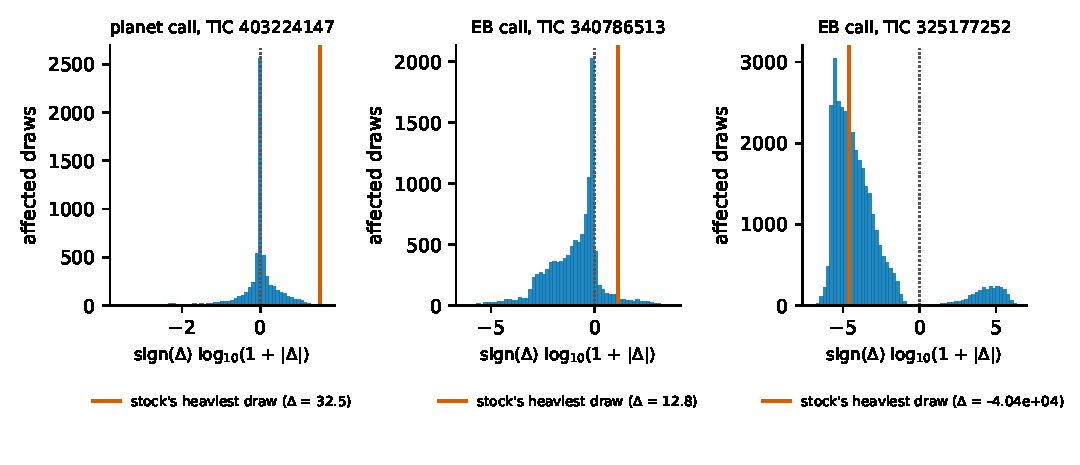
\includegraphics[width=\textwidth]{figures/fig-c-delta.pdf}
\caption{Distribution of $\Delta$, half the chi-squared of the exact curve minus that of the published code's curve, over the affected draws of a planet call of TIC 403224147, an eclipsing-binary call of TIC 340786513 (the published code higher) and an eclipsing-binary call of TIC 325177252 (the published code lower), on a signed logarithmic scale, sign$(\Delta)\log_{10}(1+|\Delta|)$. An affected draw is one on which the two curves differ by more than $10^{-6}$ at some point. Positive $\Delta$ means that the published code fits better. The vertical line is the published code's heaviest draw, the draw that carries the evidence of the call.}\label{fig:delta}
\end{figure}
% source: author's records (the Delta of every affected draw of the three calls).

\begin{figure}[ht]
\centering
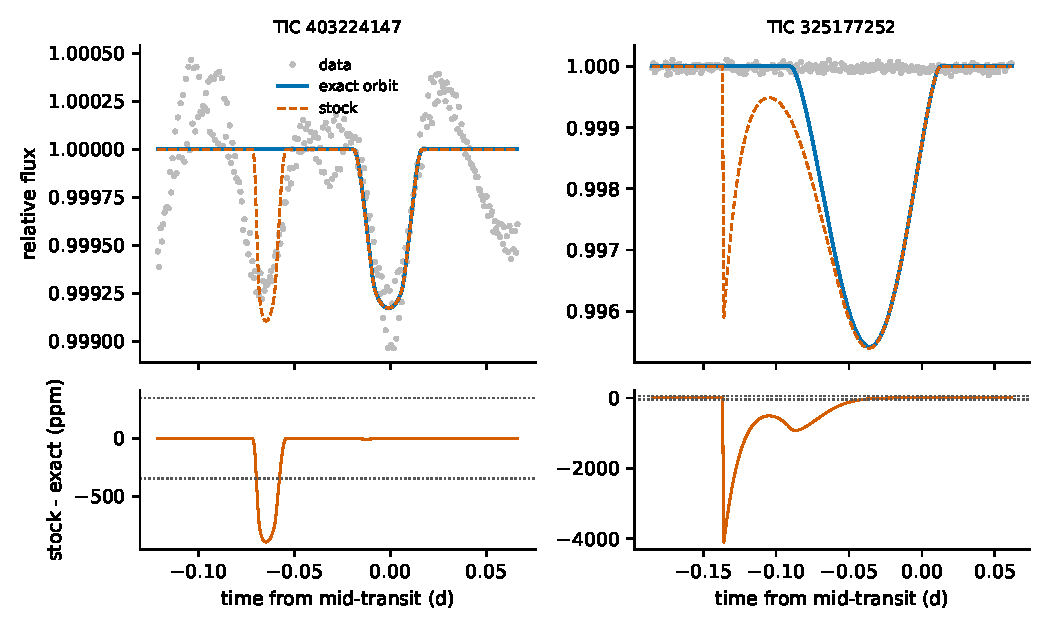
\includegraphics[width=0.95\textwidth]{figures/fig-d-curves.pdf}
\caption{The light curve of the draw that the published code weights most in the planet call of TIC 403224147 (left) and in the eclipsing-binary call of TIC 325177252 (right): the data (points), the exact curve (solid) and the published code's curve (dashed), with their difference below. The data are the binned fold of 1,000 points that the calculation uses, not binned further; the dotted lines are the noise per point, about $\pm347$ ppm on the left and $\pm50$ ppm on the right. On the left the published code has a second dip of the full depth about 0.07 d before the transit, where the exact curve is flat.}\label{fig:curves}
\end{figure}
% source: author's records (the curves of the published code's heaviest draw and the data).


\subsection{Attribution, and the shifts at $10^{6}$ draws}\label{sec:attribution}

TRICERATOPS 1.1.0 builds the \texttt{QuadraticModel} of PyTransit 2.2.0 with \texttt{interpolate=False} and calls its \texttt{evaluate\_pv} for the light curve of each draw. The orbit of that model is a Taylor expansion about mid-transit. Parviainen and Korth \cite{parviainen2020} give its accuracy near transit: the maximum error is below 1 ppm for semi-major axes larger than 5 stellar radii and for ``the major part of the physically plausible orbital parameter space'', still below 10 ppm for very eccentric orbits, and below 1 ppm ``for all but the shortest orbital periods and highest eccentricities''; their accuracy grid has periods of 2.5, 5, 15 and 30 d and $a/R_\star$ of 7.5 to 40. The draws that carry the shifts of Section~\ref{sec:model} have periods of 0.60 to 1.23 d, all below the tested range, scaled semi-major axes of 2.3 to 12.1 (five of eight under 5), eccentricities of 0.26 to 0.80, and periastron distances $a(1-e)$ of 1.4 to 3.0 stellar radii. TRICERATOPS also evaluates the curve over the whole fold, up to half a period from mid-transit, far from the point of the expansion. We read the shifts as the use of the published model beyond the range in which its authors tested it, and state it so; we did not test PyTransit inside its range, and we do not call its model defective. The cause inside the model has not been shown. A replica of the expansion, written from the text of the paper and not from the code of PyTransit, reproduces the log-likelihood of the published code to four digits on three extreme draws of two stars (TIC~42071226 and 206361339), but not on the heavy draws of TIC~201354238, where the published curve differs from the exact one by $7.0\times10^{-4}$ and $7.8\times10^{-4}$ and the replica by $1.7\times10^{-6}$ and $2.7\times10^{-6}$.
% source: Parviainen and Korth 2020 (arXiv:2009.09965; MNRAS 499, 3356), abstract and Section 4 read from the preprint (below 1 ppm for a/R* over 5; the grid of periods 2.5, 5, 15, 30 d and a/R* 7.5 to 40; below 10 ppm for very eccentric orbits; below 1 ppm for all but the shortest periods and highest eccentricities); author's records (the eight replayed heaviest draws: periods 0.604 to 1.231 d, a/R* 2.26 to 12.13, e 0.26 to 0.80; periastron distances 1.38, 1.48, 1.61, 1.82, 2.02, 2.04, 2.23 and 3.03); the author's records (the replica of the Taylor orbit: four digits on three extreme draws of TIC 42071226 and 206361339; on the heavy draws of TIC 201354238 the published curve differs from the exact by 7.0e-4 and 7.8e-4 and the replica by 1.7e-6 and 2.7e-6).

Collier et al.\ \cite{collier2026} and Giacalone et al.\ \cite{giacalone2021} run $10^{6}$ draws. Table~\ref{tab:persistence} gives FPP at that number on the same four stars, with three seeds and both calculations. The shift persists on TIC~278659026, where the FPP of the published code minus that of the default is $+0.40$ to $+0.41$, and on TIC~42071226, where it is $-0.033$ to $-0.034$, with a scatter of each calculation under 0.005 over the seeds. The side change persists on TIC~325177252: the published code stays under the line of 0.015 (0.0005 to 0.00075) and the default stays over it (0.030 to 0.032) at all three seeds. On TIC~424717049 the rule of persistence is not met: the published code gives 0.00066, 0.978 and 0.119 at its three seeds, a mean of 0.37, and the default 0.872 to 0.876; the two are on opposite sides of 0.5 at seeds 1 and 3 and on the same side at seed 2. The FPP of the published code on that star depends on the seed at $10^{6}$ draws, and that of the default does not.

\begin{table}[ht]
\centering
\caption{FPP at $10^{6}$ draws, seeds 1 to 3, of the published code and of the default of the package on the same draws. The shift persists if the difference has one sign and is at least 0.01 at all three seeds; a side change persists if the two stay on opposite sides of the line at all three seeds.}\label{tab:persistence}
\footnotesize
\begin{tabular}{lllp{3.6cm}}
\toprule
TIC & published code & default & result \\
\midrule
% source: author's records (FPP at 1e6 draws, seeds 1 to 3).
278659026 & 0.9999999785, 0.9999997808, 0.9999998249 & 0.5955, 0.5902, 0.5856 & shift persists ($+0.41$) \\
42071226 & 0.7428, 0.7359, 0.7387 & 0.7760, 0.7702, 0.7729 & shift persists ($-0.034$) \\
325177252 & 0.00051, 0.00075, 0.00052 & 0.0303, 0.0301, 0.0320 & side change of 0.015 persists \\
424717049 & 0.00066, 0.978, 0.119 & 0.8752, 0.8756, 0.8722 & rule not met \\
\bottomrule
\end{tabular}
\end{table}
% source: author's records (FPP at 1e6 draws, seeds 1 to 3, four stars; the rules; the default after the chunking of the likelihoods).


\section{Performance}\label{sec:performance}

\subsection{The card and the time of the calculation}

\paragraph{The card's rates.} On a Radeon RX 7900 XTX (ROCm 7.2) the arithmetic of one exposure node of the kernel (three small-angle Newton steps, the sky separation and the order-3 series) takes 0.534~ns per element in double precision and 0.036~ns in single precision, a ratio of 14.7. The published code on 32 CPU threads (AMD Ryzen 9 9950X3D) takes 0.89~ns per element at the same quadrature of 20 midpoints, so a double-precision kernel at the arithmetic floor of 0.53 ns would be at most about 1.7 times faster at that quadrature. No launch shape of 15 tried is faster than the default of 32 lanes in one warp, and changing the waves per execution unit from 1 to 8 changes the time by less than 1\%.
% source: author's records (0.534 ns and 0.036 ns, ratio 14.7; 0.89 ns for the published code; launch shape scan of 15 shapes).


\paragraph{The overlap and the elliptic integrals.} With three scenario calls in flight the whole calculation is 1.45 to 1.71 times faster than with one, on four stars, with the same FPP at both settings. The Landen recurrence of the elliptic integrals took at most 7 of its 8 steps in 2.1 million calls.
% source: author's records (seconds at one call in flight over seconds at three, 1.67, 1.60, 1.71 and 1.45 on four stars, FPP equal at both settings); the Landen count from the package docstring of the kernel (CEL_STEPS = 8, largest count seen 7 in 2.1 million calls).


\paragraph{What the single precision gains.} Table~\ref{tab:time} gives the time of the whole calculation on four stars, measured together with no other work on the device, medians of 5, the published code with its host-side lookups of the limb-darkening and stellar tables removed (``host fixes'') as the reference. The device in double precision at 20 midpoints is 1.33 to 2.13 times faster than the reference, with the single-precision first pass 2.27 to 3.47 times, with 3 Gauss--Legendre nodes in double precision 2.76 to 6.76 times, and at the default (3 nodes with the single-precision first pass) 3.02 to 8.59 times. The host fixes make the published code 5\% to 21\% faster. The single-precision first pass cuts the time at 20 midpoints by 20\% to 47\% and not by the factor of 14.7 of the node loop, because the Kepler solve, the tier tests and the accumulation stay in double precision and, with the single-precision first pass, 14.7\% (planet), 26.3\% (eclipsing binary) and 33.0\% (twin) of the pairs of the benchmark input need the closed form in double precision. With the node loop at the measured floor of 0.534~ns per element, the double-precision wall on the star with the most pairs flagged by the double-precision first pass is at most 1.40 times the reference, and a separate measurement of that row on the same machine was within 6\% of it.
% source: author's records (whole-calculation seconds measured together, medians of 5; ratios to the published code with the host fixes; the host fixes 5 to 21 percent; the 20 to 47 percent is 1 - mixed seconds / float64 seconds at 20 midpoints from the table) benchmarks/flagged.json (with the float32 first pass of the default: 1,470,487, 2,632,578 and 3,296,248 of 10,000,000 pairs, 14.7, 26.3 and 33.0 percent; the float64 first pass flags 8.2, 26.1 and 32.6 percent) and the author's records (ceiling 1.40 and within 6 percent, earlier measurements).

\begin{table}[ht]
\centering
\caption{Seconds of the whole calculation (medians of 5) on one AMD Radeon RX 7900 XTX and a 32-thread AMD Ryzen 9 9950X3D, measured together, at 100,000 draws. The reference is the published code with the host fixes. The last four columns are the device at 20 midpoints and at 3 nodes, each in double precision and with the single-precision first pass; the last is the default of the package. The ratio of the reference time to the row is in parentheses.}\label{tab:time}
\footnotesize
\begin{tabular}{lrrrrrr}
\toprule
TIC & published & reference & f64, 20 mid & f32, 20 mid & f64, 3 nodes & default \\
\midrule
% source: author's records (seconds of the whole calculation, medians of 5, measured together).
396212145 & 4.461 & 4.151 & 1.950 (2.13) & 1.195 (3.47) & 0.614 (6.76) & 0.483 (8.59) \\
206361339 & 1.456 & 1.155 & 0.633 (1.82) & 0.508 (2.27) & 0.419 (2.76) & 0.383 (3.02) \\
42071226  & 3.331 & 3.033 & 1.809 (1.68) & 1.112 (2.73) & 0.715 (4.24) & 0.545 (5.57) \\
201354238 & 5.548 & 5.251 & 3.954 (1.33) & 2.094 (2.51) & 1.230 (4.27) & 0.776 (6.77) \\
\bottomrule
\end{tabular}
\end{table}


The three scenario likelihoods alone, on 100,000 draws and 1,000 points, take 5.11~s with the published code on 32 threads, 4.20~s on the device in double precision at 20 midpoints, 1.90~s with the single-precision first pass, 1.02~s at 3 nodes and 0.49~s at the default, 10.35 times less than the published code.
% source: benchmarks/results.json, the block at 100,000 draws (5.1072, 4.1988, 1.8950, 1.0248 and 0.4935 seconds, the documented install); machine AMD Ryzen 9 9950X3D, RX 7900 XTX, ROCm 7.2.53211; numpy 1.26.4, torch 2.12.0+rocm7.2, triton-rocm 3.7.0, numba 0.68.1, triceratops 1.1.0, pytransit 2.2.0.


\subsection{Twenty runs of $10^{6}$ draws}

Collier et al.\ \cite{collier2026} make 20 runs of $10^{6}$ draws per target. Table~\ref{tab:cost} gives the time on one consumer card for the default of the package and for the published code on 32 CPU threads, on two stars. The published code was run at $10^{5}$ and $2\times10^{5}$ draws, because its own guard refuses a batch of draws by points larger than 2 GB, and its time and memory at $10^{6}$ draws are linear extrapolations of those two rows; its time doubles with the draws (1.97 and 2.00 times from $10^{5}$ to $2\times10^{5}$ on the two stars). The default was run at $10^{6}$ draws.
% source: author's records (the published code at 1e5 and 2e5 draws, the default at 1e5, 2e5 and 1e6, medians of 3 on TIC 396212145 and 42071226; the guard of 2 GB; 1.97 and 2.00 times a doubling).

\begin{table}[ht]
\centering
\caption{Time and memory of 20 runs of $10^{6}$ draws with the published code and with the default, on two stars, measured together after three quiet samples of the machine (medians of 3, 32 CPU threads for the published code, one AMD Radeon RX 7900 XTX with 24 GiB for the default). Measured: the published code at $10^{5}$ and $2\times10^{5}$ draws and the default at $10^{5}$, $2\times10^{5}$ and $10^{6}$ draws. Extrapolated: the run of the published code at $10^{6}$ draws, ten times its run at $10^{5}$ (the two points of each star lie on a line through the origin to within 1 percent), the 20 runs, and its memory at $10^{6}$ draws, on the line through its two points. The 20 runs of the default are 20 times its measured run. The ten batches are ten runs of $10^{5}$ draws. Device memory, with the likelihoods run in chunks, is the peak allocated by torch (\texttt{max\_memory\_allocated}) over the whole invocation, which counts tensors only and not the reserved pool, the context or the compiler.}\label{tab:cost}
\footnotesize\setlength{\tabcolsep}{4.5pt}
\begin{tabular}{lrrrrrr}
\toprule
 & \multicolumn{3}{c}{TIC 396212145} & \multicolumn{3}{c}{TIC 42071226} \\
\cmidrule(lr){2-4}\cmidrule(lr){5-7}
 & published & default & ratio & published & default & ratio \\
\midrule
% source: author's records (the rows of the table).
one run, $10^{5}$ draws (s) & 4.455 & 0.492 & 9.1 & 3.307 & 0.547 & 6.0 \\
one run, $2\times10^{5}$ draws (s) & 8.793 & 0.941 & 9.3 & 6.603 & 1.052 & 6.3 \\
one run, $10^{6}$ draws (s) & 44.6 (extrapolated) & 4.408 & 10.1 & 33.1 (extrapolated) & 5.237 & 6.3 \\
20 runs, $10^{6}$ draws (s) & 891 (extrapolated) & 88 & 10.1 & 661 (extrapolated) & 105 & 6.3 \\
ten batches of $10^{5}$ draws (s) & 44.6 & 4.92 & 9.1 & 33.1 & 5.47 & 6.0 \\
resident memory, $10^{5}$ draws (MiB) & 1,975 & 1,881 & & 2,275 & 1,891 & \\
resident memory, $10^{6}$ draws (GiB) & 6.4 (extrapolated) & 2.71 & & 9.7 (extrapolated) & 2.67 & \\
device memory, $10^{6}$ draws (GiB) & & 4.1 & & & 3.8 & \\
\bottomrule
\end{tabular}
\end{table}

The default takes 88 s and 105 s for the 20 runs of $10^{6}$ draws, 10.1 and 6.3 times less than the published code. The memory of the published code rises by 514 and 856 MiB from $10^{5}$ to $2\times10^{5}$ draws, 0.5 to 0.8 GiB per $10^{5}$ draws, so a run at $10^{6}$ draws would fit in the memory of the machine; the default needs 2.7 GiB of host memory. One run of the published code at $10^{6}$ draws was made, on a third star, TIC~325177252: 88.8 s and 11.5 GiB of resident memory, against the 33.1 and 44.6 s extrapolated for the two stars of the table, so the cost per star differs by about a factor of two on these three.
% source: author's records (88 and 105 s against 891 and 661 s; 10.1 and 6.3 times; the memory rises of 514 and 856 MiB; 2.7 GiB host) and the author's records (one the published code call at 1,000,000 draws on TIC 325177252, 88.8 s, resident memory 413 MiB before and 11,797 MiB after).

\paragraph{Device memory.} Each likelihood call holds arrays of valid draws by points in double precision, and with three calls in flight these stack. The likelihoods run in chunks of at most $2^{26}$ draws times points, which bounds a call at 1.6 GiB. With the chunks, the device peak of the default at $10^{6}$ draws is 4.1, 3.8, 4.2 and 3.9 GiB on TIC~396212145, 42071226, 325177252 and 424717049. Without the chunks the peak is 11.0 and 15.9 GiB on the first two, and on the other two the calculation runs out of memory at its first call on a card of 24 GiB, asking for 3.5 GiB with 21.3 to 21.5 GiB allocated. The chunks do not change the time: a calculation takes 4.432 and 5.267 s on the first two stars with them and 4.342 and 5.250 s without, measured together, and 12.3 and 9.1 s on the other two with them. The time depends on the star by a factor of about three at this number of draws. At $2\times10^{5}$ draws, where some calls are chunked, FPP, NFPP and all 42 scenario probabilities are equal to the last digit with and without the chunks, at three seeds, on TIC~325177252. In double precision, which the default does not use, the chunked likelihood differs from the whole in the last bit on about 1 percent of the draws, by up to $4\times10^{-12}$ relative in the log-likelihood, because the double-precision flux of a draw depends in its last bit on the other draws of its launch; the default precision is bit for bit. A user who selects double precision should expect that difference.
% source: author's records (torch.OutOfMemoryError at the first call on TIC 325177252 and 424717049, asking for 3.5 GiB with 21.3 to 21.5 GiB allocated on a card of 23.98 GiB) and the author's records (in float64 the chunked likelihood differs in the last bit on about 1 percent of draws, up to 4e-12 relative in lnL, and is bit for bit in the default precision; device peak 4,215, 3,867, 4,281 and 3,958 MiB at 1e6 draws with the chunked likelihood; before the chunks 11,243 and 16,273 MiB in the same set of measurements; seconds a calculation 4.432 and 5.267 against 4.342 and 5.250, 12.292 and 9.061; at 2e5 draws on TIC 325177252 all probabilities equal between the two codes at seeds 1 to 3).

\section{The scatter between batches}\label{sec:stating}

The scatter of the probabilities between seeds depends on the star. At $10^{5}$ draws the median scatter of FPP between ten seeds over 158 stars is 0.012, and 36 stars (0.23, Wilson 0.17 to 0.30) have a scatter over 0.05. On one star of the set, run at $10^{6}$ draws with the published code, the FPP was 0.00066, 0.978 and 0.119 at three seeds. An error stated from the sample variance of the draws does not cover the truth where one draw dominates. On seven calls of four stars it covers it in 0.08 to 0.70 of runs, for a nominal 0.90.
% source: author's records (158 stars, ten seeds, 100,000 draws: median 0.0115; 36 of 158, Wilson 0.17 to 0.30), the author's records (the published code at 1,000,000 draws, seeds 1 to 3, TIC 424717049: FPP 0.00066, 0.978, 0.119), the author's records (the published code arm, seven calls of four stars, TIC 206361339, 396212145, 177253429 and 215480963, 0.08 to 0.70).

velociraptor describes the scatter in another way. It runs a fixed number of seeded batches of $N$ draws for each scenario call, pools them into the probabilities, and reports as the error of each probability the standard deviation between batches over the root of their number, and the effective sample size $(\sum w)^{2}/\sum w^{2}$ of each call. The calls of a batch run one at a time (Section~\ref{sec:design}), and 200 of 200 evidences from 20 batches of each call, run twice at each of two settings, agree bit for bit. The coverage measurements below ran the calls of each batch one at a time. The coverage below was measured with batches of $10^{5}$ draws, so ten batches hold $10^{6}$ draws, the number of draws of one run of the published default. The coverage of a stated error is the share of runs whose interval contains the value that the error is stated for.
% source: velociraptor README, Options, and the package docstring of its allocation module (seeded batches of N draws; the error is the standard deviation between batches over the root of their number); author's records (effective sample size), the author's records (coverage), the author's records (200 of 200 evidences equal bit for bit within and between settings once the calls run one at a time, against 185 of 200 within the default and 35 of 200 against one call at a time before the change).

On the three stars where the batch count was chosen, the error covers at its nominal rate. The measurement is 40 replicates of ten batches of $10^{5}$ draws each per call, with the device calculation at 3 nodes in double precision, against the mean of 100 reference batches. The three stars have FPP of 0.02 and 0.04, near the validation line of 0.015, and 0.18. The error covers the truth in 0.925 to 0.975 of replicates for FPP and 0.90 to 0.95 for $\ln\mathrm{NFPP}$, against a nominal 0.90. The batch count was chosen on these stars, so the figures are in sample. The error does not cover where one call carries the variance. On the star whose leading call carries 0.99 of it, the coverage of $\ln\mathrm{NFPP}$ is 0.525, because the truth rests on one rare batch that the ten batches miss together. Their spread is then small and the stated error too small, with a median of 0.79 against a root mean square error of 2.22, so the error gives no warning on that star.

\paragraph{Out of sample.} Six further stars were taken by a rule that does not look at coverage: the first six in hash order whose FPP scatter over ten seeds exceeds $10^{-3}$, excluding the four stars of the measurements above (the three and the one where a call carries the variance). Each ran 100 batches of $10^{5}$ draws. Ten trials per star took a group of ten batches, the interval of $\pm1.645$ times the standard deviation over $\sqrt{10}$, and as the truth the pooled evidence of the other 90 batches. The interval contains the truth in 40 of 60 trials (0.667, Wilson 95 percent interval 0.54 to 0.77), by star 3, 10, 7, 8, 5 and 7 of 10. The interval lies entirely below the nominal 0.90, so the error taken from ten batches is not a valid 90 percent interval out of sample. Two checks made after the result, which decide nothing, do not repair it: Student's $t$ quantile at 9 degrees of freedom gives 47 of 60 (0.783, 0.66 to 0.87), and groups of 20 batches against the other 80 give 23 of 30 (0.767, 0.59 to 0.88). The effective sample size of the leading calls in the first batch is 1.3 and 3.6 on the two stars that cover 5 and 3 of 10, and 7.6 to 63.7 on the four that cover 7 to 10 of 10. This is consistent with a stated error from few batches being small where the draws that carry the evidence are rare; six stars cannot establish it. The scatter between ten batches therefore describes the Monte Carlo scatter, and a class near a decision value is unsettled where the batches straddle it.
% source: author's records (six stars by hash order; 40 of 60, 0.667, Wilson 0.541 to 0.773; by star 3, 10, 7, 8, 5, 7; post hoc t 47 of 60, 0.783, 0.664 to 0.869; 20 batches 23 of 30, 0.767, 0.591 to 0.882; ESS 1.3, 3.6, 7.6 to 63.7).
% source: author's records (40 replicates of 10 batches of 100,000 draws at 3 nodes against the mean of 100 reference batches; coverage 0.925 to 0.975 and 0.90 to 0.95; 0.525 where one call carries 0.99, median stated sd 0.793 against rms error 2.22; the stop and the gate not repairs; 0.33 to 0.58).



\paragraph{Use of the reported scatter.} The package reports the scatter between ten batches as a description of the Monte Carlo scatter of a run and states no coverage for it.

\section{Conclusions}

The exact light curve changes the result of TRICERATOPS on a minority of stars. On 15 of 158 candidates the false-positive probability or the probability of a nearby star moves by at least one seed scatter, and on two of them FPP crosses a decision value: 0.015 on one, where the published code would validate the candidate and the exact calculation would not, and 0.5 on the other (Section~\ref{sec:model}). At $10^{6}$ draws the shifts persist on three of the four stars tested, the change across 0.015 among them (Section~\ref{sec:attribution}).

The shifts come from the draws that carry the evidence of a scenario call. On those draws the light curve of PyTransit 2.2.0 is off a 50-digit reference by $4.5\times10^{-4}$ to $4.1\times10^{-3}$, at periods of 0.60 to 1.23 d and eccentricities of 0.26 to 0.80, outside the range in which its authors tested it (Section~\ref{sec:attribution}). A candidate whose scenario draws reach short, eccentric orbits is the case in which the transit model decides the result.

On one consumer card, 20 runs of $10^{6}$ draws take 88 s and 105 s on two stars, where the published code on 32 CPU threads would take an extrapolated 891 s and 661 s (Section~\ref{sec:performance}). The single-precision first pass shifts the evidence by under 0.4 percent of its seed scatter on four stars (Section~\ref{sec:fp32}).

The scatter between ten seeded batches describes the Monte Carlo scatter of a run. It covered the truth at its nominal rate on the three stars on which the batch count was chosen and in 0.667 of trials on six stars chosen by a rule that does not look at coverage, so the package states no coverage for it (Section~\ref{sec:stating}).

\section{Limits and what was not verified}\label{sec:limits}

\begin{itemize}
\item The stars are hash-ordered samples of earlier calculations (Table~\ref{tab:samples}). They are not draws from a catalog.
\item The model shift is measured on the 158 stars of the screen set that were run (Table~\ref{tab:samples}), candidates of a transit search and not stars in general or validated candidates. The published code ran at three seeds and the exact model at ten, so the shift is a mean over three paired seeds against the seed scatter of ten. The two changes of side are two cases and not a rate (Wilson interval of their share 0.35 to 4.5 percent). Two crowded fields, with more than 1,150 stars in their TRICERATOPS tables, are counted.
\item The persistence at $10^{6}$ draws is measured on four stars at three seeds. On TIC 424717049 the rule of persistence was not met, so the change of side of 0.5 on that star is not shown at that number.
\item The attribution is an argument from the range in which the accuracy of the published model was tested. The accuracy of PyTransit inside that range was not tested here, and the cause inside the model has not been shown. The three patterns of Section~\ref{sec:model} are read from the heaviest draw of the replayed calls of the shifted stars and of three controls. No pattern was tested on calls whose evidence rests on more draws, the secondary-eclipse tests inside the eclipsing-binary likelihoods were not compared, and TIC 278659026 was not replayed beyond its heaviest draws.
\item PyTransit was compared at version 2.2.0 only, with \texttt{interpolate=False} as TRICERATOPS 1.1.0 calls it. No later release and no third light-curve code was run on the same draws.
\item The coverage of the fixed batches is 0.925 to 0.975 in sample on three stars and 0.667 on six further stars; the dependence on the effective sample size rests on those six stars, fields with more than 177 stars in their tables were not measured, and no batch count that repairs the coverage was found. The scatter over many stars (Section~\ref{sec:stating}) is measured on 158 stars of one earlier set of calculations at $10^{5}$ draws, and describes that set and not TESS stars or validated candidates.
\item No reliability curve on labelled candidates has been made, and agreement of the labels with other pipelines has not been checked. The candidates with a disposition among the 158 stars were not compared with their dispositions.
\item The transit search that selected the 158 stars is not described beyond its role.
\item The speed was measured on one consumer card (Radeon RX 7900 XTX) and one CPU. The ratio of the rates in single and double precision, and the conclusions about speed, hold for this card. Data-centre cards may have a very different ratio.
\item The cost table is on two stars, medians of 3, measured together; the time and memory of the published code at $10^{6}$ draws on those two stars are extrapolated from two rows, and no run of it at $10^{6}$ draws was made on them. The comparison of the whole calculation with the published code rests on five repeats per row, measured together. Each calculation ran 100,000 draws per scenario, the number that the calling code fixes for these calculations.
\item The practice of 20 runs of $10^{6}$ draws per target is read from the text of one recent paper \cite{collier2026}; Giacalone et al.\ \cite{giacalone2021} made the 20 runs for their 12 validated objects only.
\item The product and flux column of the light curve are recorded for 136 of the 159 stars of the screen set (SPOC 2-minute, PDCSAP flux, no version tag in the file name); the other 23, from two earlier runs made before those columns were recorded, were made with the default product of the same code, and their flux column is not recorded. The TESScut cutouts and the catalogue entries of the fields are as of the day each field was built and are not versioned, so the field of a star cannot be rebuilt identically. None of the 136 recorded stars used a full-frame light curve as its light curve, and the 23 others used the default product, a 2-minute one; the pixels of every field come from full-frame cutouts. For a period in which the service gave cutouts without two header keywords, the missing keywords were set to zero, which does not change the default aperture.
\item The device memory is the peak allocated by torch; the reserved peak was not measured. The equality of the probabilities with and without the chunks was tested at $2\times10^{5}$ draws on one star; at $10^{5}$ draws no call is chunked. The cause of the dependence of the double-precision flux on the other draws of its launch is not located.
\end{itemize}


\section*{Software}

Python 3.12; NumPy 1.26 \cite{harris2020}; SciPy \cite{virtanen2020}; PyTorch 2.12 \cite{paszke2019}; Triton 3.7 \cite{tillet2019}; Numba 0.68.1 \cite{lam2015}; TRICERATOPS 1.1.0 \cite{giacalone2021,giacalone2020ascl}; PyTransit 2.2.0 \cite{parviainen2015}; mpmath 1.4 \cite{johansson2017} for the 50-digit references.
% source: versions from the benchmark record of the package (python 3.12.13, numpy 1.26.4, numba 0.68.1, torch 2.12.0+rocm7.2, triton-rocm 3.7.0, triceratops 1.1.0, pytransit 2.2.0) and the lock file of the package (mpmath 1.4.1); references checked against Crossref (Harris et al. 2020, Nature 585, 357; Virtanen et al. 2020, Nature Methods 17, 261; Tillet, Kung and Cox 2019, MAPL, pp 10-19; Lam, Pitrou and Seibert 2015, LLVM-HPC), the arXiv page of Paszke et al. (1912.01703), Zenodo for mpmath (10.5281/zenodo.1476882) and the PyPI page of TRICERATOPS (ASCL 2002.004).

\section*{Data availability}

The light curves of the targets are the 2-minute light curves of the Science Processing Operations Center (SPOC), PDCSAP flux with the default quality mask, of the Mikulski Archive for Space Telescopes (MAST), read from its public data bucket; the folded light curve that TRICERATOPS receives is made from them. The field of each calculation (the pixels around the target, the neighbouring stars and their catalogue entries) is built by TRICERATOPS itself, from cutouts of the TESS full-frame images of the same sectors obtained from the TESScut service, an aperture of 5 by 5 pixels centred on the target, the TESS Input Catalog and Gaia catalogues, and a Gaia background population, as they were on the day of the first calculation of each star. The package, its tests and the validation scripts are at \texttt{https://github.com/mauri870/velociraptor}. The records of the measurements of this paper other than the benchmarks and the validation of the package are available from the author on request.
% source: the loading of the light curves for these calculations (the 2-minute SPOC product of the public bucket stpubdata, files ending in s_lc.fits; the default product when the configuration names none; the flux column and product are recorded in its stored rows: SPOC and pdcsap_flux on 136 of the 159 stars of the screen set, no record on 23) and its call of TRICERATOPS (the target built by TRICERATOPS 1.1.0 from lightkurve's TESScut cutouts, the default aperture of 5 by 5 pixels, the TIC and Gaia catalogues, the setting to zero of two header keywords missing from some cutouts, the field saved at the first call).

\appendix
\section{The 158 stars of the model comparison}\label{sec:stars}

Table~\ref{tab:stars} lists the 158 stars of the comparison of Section~\ref{sec:model}. FPP is the mean over seeds 1 to 3 of the published code and of the exact model on the same draws. A star is shifted under the rule of Section~\ref{sec:model}, in FPP, in $\ln\mathrm{NFPP}$ or in both.
% source: author's records (the per-star table of the comparison: stratum, the means of FPP over the three paired seeds, the shifts and the changes of side).

\begin{center}
\scriptsize
\setlength{\tabcolsep}{3.5pt}\setlength{\LTcapwidth}{\textwidth}
\begin{longtable}{rllll@{\hspace{2.5em}}rllll}
\caption{The stars of the model comparison. Stratum F is flagged by the screen of Table~\ref{tab:samples} and N is not. FPP is the mean over three seeds of the published code (pub.) and of the exact model (exact) on the same draws. A dagger marks the two stars whose FPP changes side of 0.015 or 0.5.}\label{tab:stars}\\
\toprule
TIC & stratum & FPP pub. & FPP exact & shifted & TIC & stratum & FPP pub. & FPP exact & shifted \\
\midrule
\endfirsthead
\toprule
TIC & stratum & FPP pub. & FPP exact & shifted & TIC & stratum & FPP pub. & FPP exact & shifted \\
\midrule
\endhead
\bottomrule
\endfoot
26584326 & F & 0.755 & 0.763 &  & 231694736 & N & 0.300 & 0.288 &  \\
32052779 & F & 1.000 & 1.000 &  & 233680140 & N & $>0.999$ & $>0.999$ &  \\
38516712 & F & 0.333 & 0.333 &  & 234291977 & N & 0.561 & 0.559 &  \\
40339576 & F & 0.214 & 0.214 &  & 237158650 & N & 0.694 & 0.694 &  \\
42071226 & F & 0.739 & 0.775 & FPP & 237325365 & N & $>0.999$ & $>0.999$ &  \\
122609268 & F & 1.000 & 1.000 &  & 243354593 & N & $>0.999$ & $>0.999$ &  \\
122609480 & F & $>0.999$ & 0.895 & FPP & 256865831 & N & $>0.999$ & $>0.999$ &  \\
150431617 & F & $>0.999$ & $>0.999$ &  & 259719464 & N & 0.246 & 0.246 &  \\
166732511 & F & 0.376 & 0.374 &  & 261526008 & N & $3.2\times10^{-10}$ & $1.3\times10^{-10}$ &  \\
167303776 & F & 1.000 & 1.000 &  & 262818577 & N & 0.556 & 0.557 &  \\
193318850 & F & 0.262 & 0.263 &  & 265438551 & N & 0.032 & 0.028 & NFPP \\
197949562 & F & 0.049 & 0.049 &  & 265588613 & N & 0.045 & 0.045 &  \\
201233593 & F & $3.5\times10^{-4}$ & $3.5\times10^{-4}$ &  & 278659026 & N & $>0.999$ & 0.577 & FPP, NFPP \\
201235927 & F & 0.251 & 0.251 &  & 292292315 & N & 1.000 & 1.000 &  \\
229796245 & F & 0.999 & 0.999 &  & 293419639 & N & 1.000 & 1.000 &  \\
231670778 & F & 1.000 & 1.000 &  & 294198241 & N & 0.438 & 0.452 &  \\
231910539 & F & 0.999 & 0.999 &  & 295615371 & N & 1.000 & 1.000 &  \\
238815210 & F & 0.333 & 0.333 &  & 296739893 & N & 0.997 & 0.997 &  \\
261460023 & F & 0.988 & 0.988 &  & 302107568 & N & 0.056 & 0.056 &  \\
288344202 & F & 1.000 & 1.000 &  & 311401333 & N & 0.141 & 0.141 &  \\
292542560 & F & 1.000 & 1.000 &  & 311893557 & N & 1.000 & 1.000 &  \\
294884819 & F & 1.000 & 1.000 &  & 314864866 & N & 0.999 & 0.999 &  \\
300010099 & F & 1.000 & 1.000 &  & 316787978 & N & 0.096 & 0.096 &  \\
302061421 & F & 1.000 & 1.000 &  & 316936115 & N & 0.881 & 0.880 &  \\
340786513 & F & $>0.999$ & 0.806 & FPP & 318566416 & N & 0.124 & 0.124 &  \\
343886954 & F & 0.208 & 0.207 &  & 321908598 & N & 1.000 & 1.000 &  \\
345088232 & F & $>0.999$ & 0.991 &  & 321908619 & N & 1.000 & 1.000 &  \\
355547387 & F & 1.000 & 1.000 &  & 325177252 & N & $8.6\times10^{-4}$ & 0.034 & FPP$^{\dagger}$ \\
360918475 & F & 1.000 & 1.000 &  & 325210265 & N & 0.946 & 0.940 &  \\
361281902 & F & 0.198 & 0.198 &  & 325338668 & N & 1.000 & 1.000 &  \\
382575967 & F & 1.000 & 1.000 &  & 327724364 & N & 0.359 & 0.359 &  \\
389021976 & F & 1.000 & 1.000 &  & 328100489 & N & 0.911 & 0.911 &  \\
389752750 & F & 1.000 & 1.000 &  & 340003212 & N & 1.000 & 1.000 &  \\
391903064 & F & 1.000 & 1.000 &  & 340878553 & N & 1.000 & 1.000 &  \\
394557413 & F & 1.000 & 1.000 &  & 341497604 & N & 0.945 & 0.945 &  \\
402546736 & F & 0 & $2.4\times10^{-14}$ &  & 343647193 & N & 1.000 & 1.000 &  \\
403224147 & F & $>0.999$ & 0.701 & FPP & 343887624 & N & 1.000 & 1.000 &  \\
405410684 & F & $>0.999$ & 0.885 & FPP & 347030355 & N & 0.179 & 0.178 &  \\
406322391 & F & 0.020 & 0.020 &  & 350222730 & N & 1.000 & 1.000 &  \\
410148949 & F & 1.000 & 1.000 &  & 354654467 & N & 1.000 & 1.000 &  \\
410214986 & F & 0 & 0 &  & 358516596 & N & 0.847 & 0.836 & FPP \\
425884522 & F & 0.152 & 0.152 &  & 359497943 & N & 0.076 & 0.074 &  \\
425923664 & F & 1.000 & 1.000 &  & 360453460 & N & 1.000 & 1.000 &  \\
466094094 & F & 0.193 & 0.192 &  & 365660822 & N & $>0.999$ & 0.973 & NFPP \\
2055541811 & F & 0.994 & 0.994 &  & 369964729 & N & $5.4\times10^{-4}$ & $5.4\times10^{-4}$ &  \\
13574905 & N & 0.871 & 0.873 &  & 373431424 & N & $>0.999$ & $>0.999$ &  \\
26826078 & N & 0.994 & 0.994 &  & 375506058 & N & 0.333 & 0.333 &  \\
55652896 & N & 0.667 & 0.667 &  & 376669357 & N & 1.000 & 1.000 &  \\
69679391 & N & 0 & 0 &  & 377292556 & N & 0.485 & 0.485 &  \\
69747919 & N & 0.465 & 0.443 &  & 382039146 & N & 0.574 & 0.599 & NFPP \\
73644471 & N & 0.360 & 0.360 &  & 382384315 & N & 1.000 & 1.000 &  \\
101944811 & N & 0.107 & 0.107 &  & 391880567 & N & 0.706 & 0.707 &  \\
139370537 & N & 0.204 & 0.204 &  & 391949880 & N & 0.104 & 0.104 &  \\
140889223 & N & 0.989 & 0.989 &  & 392747437 & N & 0.790 & 0.790 &  \\
141975044 & N & 0.155 & 0.155 &  & 393977332 & N & 1.000 & 1.000 &  \\
146320244 & N & 0.096 & 0.096 &  & 396211656 & N & 1.000 & 1.000 &  \\
150391436 & N & 0.644 & 0.667 & NFPP & 396212145 & N & 1.000 & 1.000 &  \\
155896956 & N & 0.051 & 0.051 &  & 401827140 & N & 0.140 & 0.140 &  \\
158324245 & N & 0 & 0 &  & 402046099 & N & 1.000 & 1.000 &  \\
160220653 & N & 1.000 & 1.000 &  & 402972169 & N & 1.000 & 1.000 &  \\
161378663 & N & 0.104 & 0.104 &  & 403121375 & N & 0.015 & 0.014 &  \\
163029327 & N & 0.018 & 0.018 &  & 405411672 & N & 1.000 & 1.000 &  \\
165124221 & N & 0.214 & 0.199 & FPP & 407575998 & N & 0.006 & 0.006 &  \\
165145322 & N & 1.000 & 1.000 &  & 408310006 & N & 0.931 & 0.931 &  \\
169556484 & N & 0.524 & 0.524 &  & 410056850 & N & 0.005 & 0.005 &  \\
177253429 & N & $>0.999$ & $>0.999$ &  & 410118578 & N & 1.000 & 1.000 &  \\
179582003 & N & 0.996 & 0.996 &  & 410402714 & N & 0.279 & 0.279 &  \\
198354567 & N & 0.253 & 0.253 &  & 417679385 & N & 0.558 & 0.518 & FPP \\
201252144 & N & 0.674 & 0.674 &  & 417931607 & N & 0.087 & 0.087 &  \\
201288535 & N & 1.000 & 1.000 &  & 421184129 & N & 0.017 & 0.017 &  \\
201289552 & N & 0.443 & 0.443 &  & 421472503 & N & 0.052 & 0.052 &  \\
201306147 & N & 0.646 & 0.646 &  & 424717049 & N & 0.104 & 0.877 & FPP$^{\dagger}$ \\
206288957 & N & 0.643 & 0.641 &  & 448714306 & N & 0.284 & 0.284 &  \\
206361339 & N & 0.268 & 0.268 &  & 448922221 & N & 1.000 & 1.000 &  \\
215480963 & N & 0.800 & 0.800 &  & 449114791 & N & 1.000 & 1.000 &  \\
219327284 & N & 0.190 & 0.190 &  & 466095512 & N & 1.000 & 1.000 &  \\
220021331 & N & 0.765 & 0.765 &  & 466131866 & N & 1.000 & 1.000 &  \\
229152539 & N & 0.082 & 0.082 &  & 466207143 & N & 1.000 & 1.000 &  \\
230086768 & N & 1.000 & 1.000 &  & 2026649904 & N & $>0.999$ & $>0.999$ &  \\
\end{longtable}
\end{center}

\begin{thebibliography}{99}
\bibitem{giacalone2021} Giacalone, S., Dressing, C. D., Jensen, E. L. N., et al. 2021, Vetting of 384 TESS Objects of Interest with TRICERATOPS and Statistical Validation of 12 Planet Candidates, AJ, 161, 24, \texttt{arXiv:2002.00691}
\bibitem{morton2012} Morton, T. D. 2012, An Efficient Automated Validation Procedure for Exoplanet Transit Candidates, ApJ, 761, 6, \texttt{arXiv:1206.1568}
\bibitem{morton2016} Morton, T. D., Bryson, S. T., Coughlin, J. L., et al. 2016, False Positive Probabilities for all Kepler Objects of Interest: 1284 Newly Validated Planets and 428 Likely False Positives, ApJ, 822, 86, \texttt{arXiv:1605.02825}
\bibitem{diaz2014} D\'iaz, R. F., Almenara, J. M., Santerne, A., et al. 2014, PASTIS: Bayesian extrasolar planet validation. I. General framework, models, and performance, MNRAS, 441, 983, \texttt{arXiv:1403.6725}
\bibitem{torres2011} Torres, G., Fressin, F., Batalha, N. M., et al. 2011, Modeling Kepler transit light curves as false positives: Rejection of blend scenarios for Kepler-9, and validation of Kepler-9d, a super-Earth-size planet in a multiple system, ApJ, 727, 24, \texttt{arXiv:1008.4393}
\bibitem{mandel2002} Mandel, K., \& Agol, E. 2002, Analytic Lightcurves for Planetary Transit Searches, ApJ, 580, L171, \texttt{arXiv:astro-ph/0210099}
\bibitem{agol2020} Agol, E., Luger, R., \& Foreman-Mackey, D. 2020, Analytic Planetary Transit Light Curves and Derivatives for Stars with Polynomial Limb Darkening, AJ, 159, 123
\bibitem{parviainen2015} Parviainen, H. 2015, MNRAS, 450, 3233
\bibitem{parviainen2020} Parviainen, H., \& Korth, J. 2020, Going back to basics: accelerating exoplanet transit modelling using Taylor-series expansion of the orbital motion, MNRAS, 499, 3356, \texttt{arXiv:2009.09965}
\bibitem{collier2026} Collier, M., Giacalone, S., Derfer, B., et al. 2026, Assessing the Impact of High-Resolution Imaging on Statistical Validation of TESS Planet Candidates, \texttt{arXiv:2608.21560}
\bibitem{harris2020} Harris, C. R., Millman, K. J., van der Walt, S. J., et al. 2020, Array programming with NumPy, Nature, 585, 357, \texttt{doi:10.1038/s41586-020-2649-2}
\bibitem{virtanen2020} Virtanen, P., et al. 2020, SciPy 1.0: fundamental algorithms for scientific computing in Python, Nature Methods, 17, 261, \texttt{doi:10.1038/s41592-019-0686-2}
\bibitem{paszke2019} Paszke, A., et al. 2019, PyTorch: An Imperative Style, High-Performance Deep Learning Library, Advances in Neural Information Processing Systems 32, \texttt{arXiv:1912.01703}
\bibitem{tillet2019} Tillet, P., Kung, H. T., \& Cox, D. 2019, Triton: an intermediate language and compiler for tiled neural network computations, Proceedings of the 3rd ACM SIGPLAN International Workshop on Machine Learning and Programming Languages, 10, \texttt{doi:10.1145/3315508.3329973}
\bibitem{lam2015} Lam, S. K., Pitrou, A., \& Seibert, S. 2015, Numba: a LLVM-based Python JIT compiler, Proceedings of the Second Workshop on the LLVM Compiler Infrastructure in HPC, \texttt{doi:10.1145/2833157.2833162}
\bibitem{johansson2017} Johansson, F., et al., mpmath: a Python library for arbitrary-precision floating-point arithmetic, Zenodo, \texttt{doi:10.5281/zenodo.1476882}
\bibitem{giacalone2020ascl} Giacalone, S., \& Dressing, C. D. 2020, triceratops: Candidate exoplanet rating tool, Astrophysics Source Code Library, \texttt{ascl:2002.004}
\end{thebibliography}

\end{document}
